\documentclass[11pt, a4paper]{article}
    %\usepackage{geometry}
    \usepackage[inner=1.5cm,outer=1.5cm,top=2.5cm,bottom=2.5cm]{geometry}
    \pagestyle{empty}
    \usepackage{graphicx}
    \usepackage{fancyhdr, lastpage, bbding, pmboxdraw}
    \usepackage[usenames,dvipsnames]{color}
    \definecolor{darkblue}{rgb}{0,0,.6}
    \definecolor{darkred}{rgb}{.7,0,0}
    \definecolor{darkgreen}{rgb}{0,.6,0}
    \definecolor{red}{rgb}{.98,0,0}
    \usepackage[colorlinks,pagebackref,pdfusetitle,urlcolor=darkblue,citecolor=darkblue,linkcolor=darkred,bookmarksnumbered,plainpages=false]{hyperref}
    \renewcommand{\thefootnote}{\fnsymbol{footnote}}
    
    \pagestyle{fancyplain}
    \fancyhf{}
    \lhead{ \fancyplain{}{Oil Digger} }
    \rhead{ \fancyplain{}{CSCI 470 - Project Progress Report} }
    %\rfoot{\fancyplain{}{page \thepage\ of \pageref{LastPage}}}
    % \fancyfoot[RO, LE] {page \thepage\ of \pageref{LastPage} }
    \thispagestyle{plain}
    
    %%%%%%%%%%%% LISTING %%%
    \usepackage{listings}
    \usepackage{caption}
    \DeclareCaptionFont{white}{\color{white}}
    \DeclareCaptionFormat{listing}{\colorbox{gray}{\parbox{\textwidth}{#1#2#3}}}
    \captionsetup[lstlisting]{format=listing,labelfont=white,textfont=white}
    \usepackage{verbatim} % used to display code
    \usepackage{fancyvrb}
    \usepackage{acronym}
    \usepackage{amsthm}
    \VerbatimFootnotes % Required, otherwise verbatim does not work in footnotes!
    
    \usepackage{booktabs}
    
    \definecolor{OliveGreen}{cmyk}{0.64,0,0.95,0.40}
    \definecolor{CadetBlue}{cmyk}{0.62,0.57,0.23,0}
    \definecolor{lightlightgray}{gray}{0.93}
    
    
    
    \lstset{
    %language=bash,                          % Code langugage
    basicstyle=\ttfamily,                   % Code font, Examples: \footnotesize, \ttfamily
    keywordstyle=\color{OliveGreen},        % Keywords font ('*' = uppercase)
    commentstyle=\color{gray},              % Comments font
    numbers=left,                           % Line nums position
    numberstyle=\tiny,                      % Line-numbers fonts
    stepnumber=1,                           % Step between two line-numbers
    numbersep=5pt,                          % How far are line-numbers from code
    backgroundcolor=\color{lightlightgray}, % Choose background color
    frame=none,                             % A frame around the code
    tabsize=2,                              % Default tab size
    captionpos=t,                           % Caption-position = bottom
    breaklines=true,                        % Automatic line breaking?
    breakatwhitespace=false,                % Automatic breaks only at whitespace?
    showspaces=false,                       % Dont make spaces visible
    showtabs=false,                         % Dont make tabls visible
    columns=flexible,                       % Column format
    morekeywords={__global__, __device__},  % CUDA specific keywords
    }
    
    %%%%%%%%%%%%%%%%%%%%%%%%%%%%%%%%%%%%
    \begin{document}

    \begin{titlepage}
        \begin{center}
            \vspace*{2in}
            {\Large \textsc{Project Progress Report}}\\
            \vspace*{0.1in}
 	{\Large \textsc{Identifying Sweet Spots Using Well Log Datasets}}\\
            \vspace*{0.1in}
            CSCI 470: Introduction to Machine Learning\\
            \vspace*{0.1in}
            \date{\today}
            
            \vspace*{3in}
            \large{\textbf{Team Name: Oil Digger}} \\
            \vspace*{0.1in}
            % Sort by alphabetical order of last names
            \large{Nadima Dwihusna} \\
            \vspace*{0.1in}
            \large{Xiaoyu (Rosie) Zhu} \\
            \vspace*{0.1in}
            \large{Mohamed Ibrahim Mohamed} \\
        \end{center}
    \end{titlepage}
    


    % Restate the proposed timeline and individual task assignment
    \noindent\textbf{Original Timeline} \\
    \begin{minipage}[t]{\textwidth}
        \begin{center}
        	\begin{tabular}{cccc}
                	\toprule
                	Week Starting & Nadima Dwihusna&Xiaoyu (Rosie) Zhu&Mohamed Mohamed  \\
                	\midrule
               		9/17 &  Obtain Data Sets & Obtain Data Sets and Research & Research on ML Methods\\
                	\hline
                	9/24 &  Data Processing & Data Visualization & Research on ML Methods\\
                	\hline
                	10/1 & Data Processing &Data Visualization& Research on ML Methods\\
                	\hline
                	10/8 & Data Processing & Data Visualization & ML Method Selection\\
                	\hline
                	10/15 & & All: Progress Report (Due Oct18) & \\
                	\hline
                	10/22 & Data Training & Data Prediction & Help Team Members  \\
                	\hline
                	10/29 & Data Training & Data Prediction & Help Team Members \\
                	\hline
                	11/5 & ML Method 1 & ML Method 2 & ML Method 3 \\
                	\hline
                	11/12 & ML Method 1 & ML Method 2 & ML Method 3 \\
                	\hline
                	11/19 & ML Method 1 & ML Method 2 & ML Method 3 \\
                	\hline
                	11/26 & & All: Visualize Results with Seismic & \\
                	\hline
                	12/3 & & All: Prepare Final Presentation& \\
                	\bottomrule
            \end{tabular}
        \end{center}
    \end{minipage}


    \vskip.15in

    \noindent\textbf{Objective:} 

\noindent The main goal of this project is to use Supervised Machine Learning Algorithms to identify the formation bearing fluids (Oil, Gas, and Water). Identifying these bearing fluids has been common in the oil and gas industry. However, this has been done manually for the past decades. Manual identification of sweet spots can result in many errors as human or user errors and moreover manual identification overlooks the instrumental errors, environmental disturbance and units inconsistency. The code could be further develop to determine compaction and depth trends per facies by analyzing larger scale heterogeneous datasets. The end result will be useful for rock physics and inversion workflow to improve reservoir characterization.

    % Practical Progress Report Template
    \vskip.15in
    % Mention the finalized dataset you will be using. Provide urls to the data.
    \noindent\textbf{Data:}

\noindent Database is provided by the Reservoir Characterization Project (RCP), geophysics research group at the Colorado School of Mines. The well log datasets are in the Wattenberg Field, Colorado located south of Greeley and north of Brighton, Colorado. All data is labeled and the machine learning algorithm in this project aims to inherent structure from the input data. The four well log datasets to be used are:
\begin{itemize}
	\item Badding USX W
	\vskip.0005in
	\item Warner 16-14
	\vskip.0005in
	\item Badding 15-26
	\vskip.0005in
	\item Badding 20-26
\end{itemize}


    \vskip.15in
    % Describe the features from the data and from extraction that you plan on using
    % Remove this section if Theory Project
    \noindent\textbf{Features Used:} 

\noindent The well log datasets contain several records throughout depth. Each record includes the well Name, as well as the Depth (ft) of the readings, and the following features:
\begin{itemize}
	\item \textbf{Gamma Ray (api):} measure the natural radioactivity of a rock formation to distinguish between shale and non-shale rock formations useful to indicate top of oil reservoir.
	\item \textbf{Resistivity (siemens/m):} measures how much sediments in the formation opposes electric current useful to indicate porosity of formation, water saturation, and presence of hydrocarbons.
	\item \textbf{Neutron Porosity (percent):} indicates the porosity or the void fraction in the formation; typically hydrocarbons are present in higher porosity zones.
	\item \textbf{Density (g/cc):} measures the bulk density of the formation which includes minerals and fluid.
	\item \textbf{Sonic P and Sonic S:} measures wave velocity for seismic profiles.

\end{itemize}


    \vskip.15in
    % Describe the current model you are using, and any preliminary results that you have from it
    \noindent\textbf{Current Model:} 

\noindent For this progress report, we performed data processing and visualization. We label the data with 0, 1, 2 stand for oil, water and gas, and plot the 5 features and target of all 4 wells. In this project, we decided to use supervised learning to get our target which is the Hydrocarbons types; (Oil, water or gas). As we have 5 features in the data, we are also going to perform autoencoder or PCA to extract the features.
We used three algorithms to predict our labels. First we used Support vector Machine, where we also iterated to obtain the best parameters for the model naming gamma and C (Cross Validation). Second we used Random Forest Classifier and finally we used K nearest neighbor where we also iterated the to get the best k values. Below the well log datasets are visualized along with the labeled interpreted formation bearing fluids.

\begin{figure}[h!]
  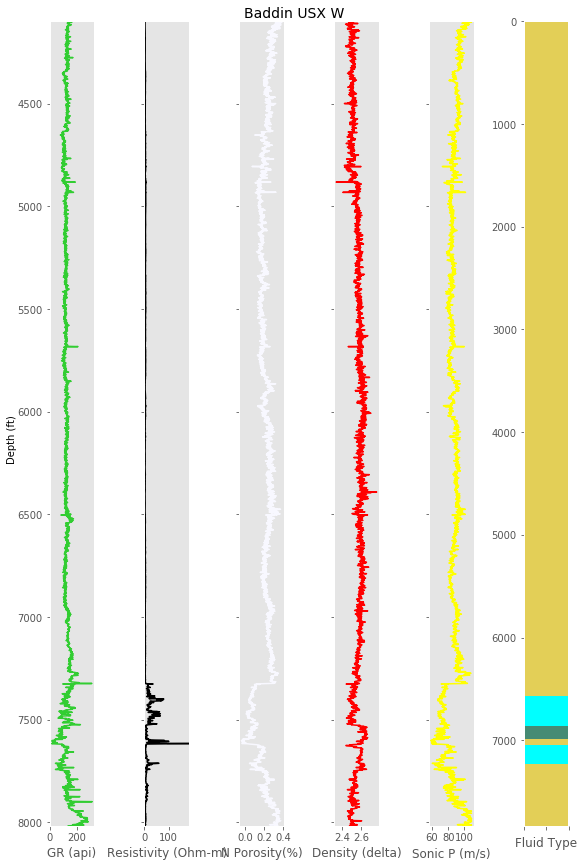
\includegraphics[width=\linewidth]{w1}
 % \caption{A boat.}
 % \label{fig:boat1}
\end{figure}
   \begin{figure}[h!]
  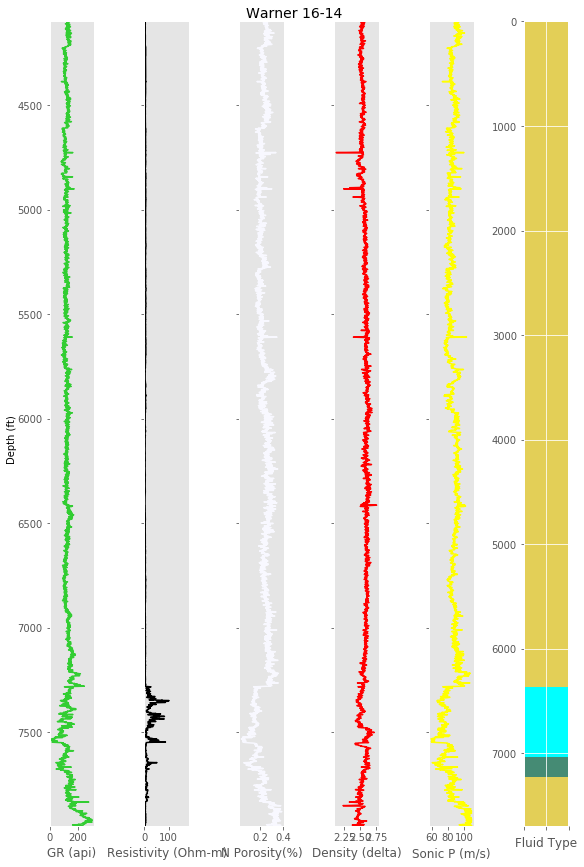
\includegraphics[width=\linewidth]{w2}
 % \caption{A boat.}
 % \label{fig:boat1}
\end{figure}
\begin{figure}[h!]
  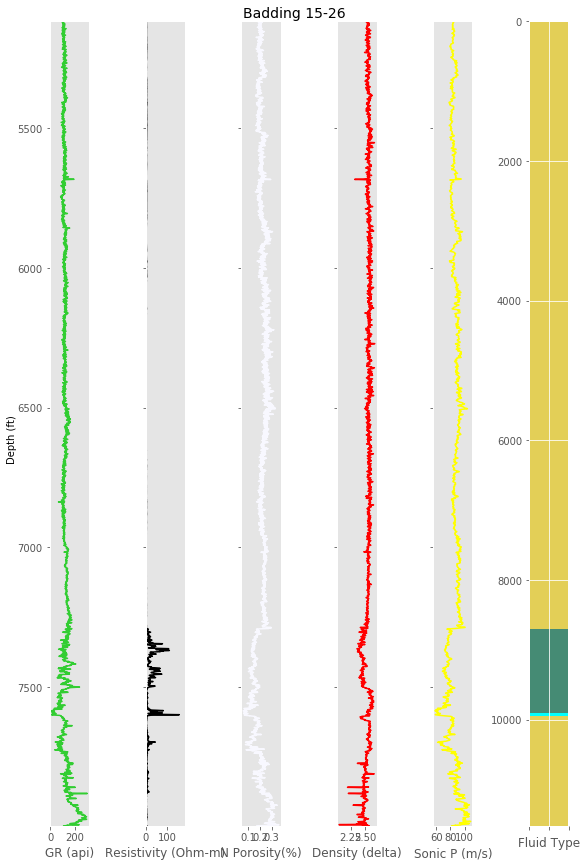
\includegraphics[width=\linewidth]{w3}
 % \caption{A boat.}
 % \label{fig:boat1}
\end{figure}
\begin{figure}[h!]
  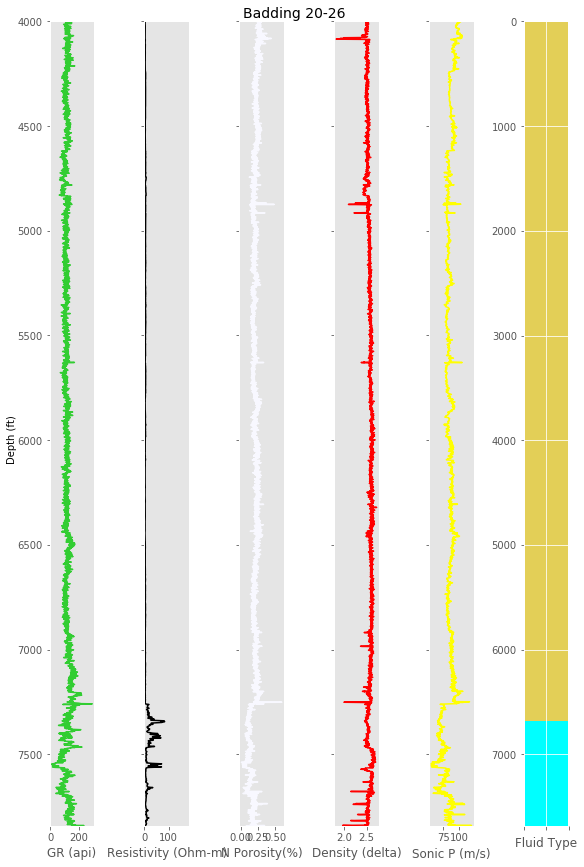
\includegraphics[width=\linewidth]{w4}
 % \caption{A boat.}
 % \label{fig:boat1}
\end{figure}

    \vskip.15in
    % Describe the actual timeline based on what you actually got done
    \noindent\textbf{Actual Timeline} 
\noindent As of now, Oil Digger group is on track with the original proposed timeline. The Wattenberg Field well log datasets were obtained, processed, and visualized preliminary research regarding the geology of datasets were analyzed, and the different Unsupervised Machine Learning Algorithms to be used were determined. The group will continue on with the timeline, training the data and performing the different algorithms.
 \vskip.15in
    \noindent\begin{minipage}[t]{\textwidth}
        \begin{center}
        	\begin{tabular}{cccc}
                	\toprule
                	Week Starting & Nadima Dwihusna&Xiaoyu (Rosie) Zhu&Mohamed Mohamed  \\
                	\midrule
               		9/17 &  Obtain Data Sets & Obtain Data Sets and Research & Research on ML Methods\\
                	\hline
                	9/24 &  Data Processing & Data Visualization & Research on ML Methods\\
                	\hline
                	10/1 & Data Processing &Data Visualization& Research on ML Methods\\
                	\hline
                	10/8 & Data Processing & Data Visualization & ML Method Selection\\
                	\hline
                	10/15 & & All: Progress Report (Due Oct18) & \\
                	\hline
                	10/22 & Data Training & Data Prediction & Help Team Members  \\
                	\hline
                	10/29 & Data Training & Data Prediction & Help Team Members \\
                	\hline
                	11/5 & ML Method 1 & ML Method 2 & ML Method 3 \\
                	\hline
                	11/12 & ML Method 1 & ML Method 2 & ML Method 3 \\
                	\hline
                	11/19 & ML Method 1 & ML Method 2 & ML Method 3 \\
                	\hline
                	11/26 & & All: Visualize Results with Seismic & \\
                	\hline
                	12/3 & & All: Prepare Final Presentation& \\
                	\bottomrule
            \end{tabular}
        \end{center}
    \end{minipage}

    \vskip.15in
    % Describe any issues that came up and how you intend to deal with them
    \noindent\textbf{Issues, Constraints \& Mitigation Strategies:} 

\noindent There are no issues that came up thus far. For the future, we plan to do further supervised learning algorithms and develop the code even more to us machine learning to identify the formation bearing fluids.

    \vskip.15in
    % Describe your new expectations for the project
    \noindent\textbf{Updated Project Expectation and Future Timeline:} 


    % Describe the timeline for the future given the way things have turned out

\noindent The Oil Digger group will continue on with the original timeline, training the data and performing the different algorithms. The future project expectation will take approximately six more weeks until all the results are obtained and visualized along a possible Seismic Profile for further accurate geological interpretation.

 \vskip.15in
    \noindent \begin{minipage}[t]{\textwidth}
        \begin{center}
        	\begin{tabular}{cccc}
                	\toprule
                	Week Starting & Nadima Dwihusna&Xiaoyu (Rosie) Zhu&Mohamed Mohamed  \\
                	\hline
                	10/22 & Data Training & Data Prediction & Help Team Members  \\
                	\hline
                	10/29 & Data Training & Data Prediction & Help Team Members \\
                	\hline
                	11/5 & ML Method 1 & ML Method 2 & ML Method 3 \\
                	\hline
                	11/12 & ML Method 1 & ML Method 2 & ML Method 3 \\
                	\hline
                	11/19 & ML Method 1 & ML Method 2 & ML Method 3 \\
                	\hline
                	11/26 & & All: Visualize Results with Seismic & \\
                	\hline
                	12/3 & & All: Prepare Final Presentation& \\
                	\bottomrule
            \end{tabular}
        \end{center}
    \end{minipage}
        %%%%%% THE END 
    \end{document} 